%!TEX root = ../dissertation.tex
% this file is called up by thesis.tex
% content in this file will be fed into the main document

%: ----------------------- introduction file header -----------------------
% the code below specifies where the figures are stored
\graphicspath{{2-deeplearning/figures/}}

\chapter{Deep Learning in a Nutshell}\label{sec:deeplearning}
\label{ch:deeplearning}

Since recently, a family of machine learning research under the buzzword \emph{deep learning} has incurred many groundbreaking changes to the world of artificial intelligence, making the long-waited dream of the artificial general intelligence look not so distant in the future.
The impact of deep learning was so dramatic that many successful applications of deep learning like DeepMind's AlphaGo outplaying the human Go champion and Google's neural machine translation have became familiar to the general public.
The core idea of using artificial neural networks to process complex information traces back to the earliest days of computing \cite{kleene1951representation}, but it has long been considered less effective than alternative methods, such as support vector machines or probabilistic graphical models.
Since around 2010, it has been increasingly shown that neural networks can substantially outperform those other approaches and have much more capability for further improvements, and that the lower performance of neural networks in the past was merely due to insufficient data, the lack of computational power, and some numerical tricks that have not been employed before.
This finding has opened the era of deep learning, a term coined after the fact that neural networks often employ multiple layers of learned feature transformations, and is continuing to innovate virtually all fields of science and engineering, including, of course, music technology.

This chapter reviews the essential concepts and terminologies of deep learning, from the basic architectures and techniques to the most recent advances in deep generative models.
The purpose of this chapter is to provide a historical perspective towards deep latent variable models and put deep generative models into the context of the proposed research on automatic music transcription.


\section{Neural Network Architectures}

The key idea of an artificial neural network in the simplest setting is to find an appropriate matrix $W$ to model the relationship between variables $\mathbf{x}$ and $\mathbf{y}$, so that
\begin{equation}\label{eqn:perceptron}
	\mathbf{y} = \sigma(W \mathbf{x})
\end{equation}
is a good approximation, where $\sigma$ is a nonlinear function like the sigmoid or the hyperbolic tangent.
This model in Equation \ref{eqn:perceptron} is also known as a perceptron \cite{rosenblatt1957perceptron}, one of the first artificial neural networks in history.
This computation --- a matrix multiplication followed by a nonlinear activation --- can be applied multiple times, like
\begin{equation}\label{eqn:mlp}
	\mathbf{y} = \sigma(W_3\sigma(W_2 \sigma(W_1 \mathbf{x})))
\end{equation}
which gives the model more expressive power.
This model in Equation \ref{eqn:mlp} is called a multilayer perceptron (MLP) in a sense that it is a concatenation of perceptrons, and the fact that it contains multiple layers is why these neural networks are called ``deep".


A multilayer perceptron is a special case of feedforward neural networks, which refer to any computational graph that does not contain a cycle.
A popular model under this category is \emph{convolutional neural networks} (CNN), which uses a convolution (a cross-correlation, to be precise) with fixed-size kernels instead of the fully connected layers performing matrix multiplications.
A 2-D convolutional layer takes input arrays $X_c \in \mathbb{R}^{H \times W}$, $c \in \{ 1, \cdots, C \}$, and produces output arrays $Y_d \in \mathbb{R}^{H \times W}$, $d \in \{ 1, \cdots, D \}$.
The kernels $K_{cd} \in \mathbb{R}^{K_1 \times K_2}$, $c \in \{ 1, \cdots, C \}$, $d \in \{ 1, \cdots, D \}$, and the biases $\mathbf{b} \in \mathbb{R}^D$ are the parameters to be optimized, and the output is calculated as:
\begin{equation}\label{eqn:convnet}
Y_{d}[i,~j] = \sum_{m=1}^{K_1} \sum_{n=1}^{K_2} \sum_{c=1}^C K_{cd}[m,~n] X_c[i+m,~j+n] + b_d
\end{equation}
There are various options to this operation including whether to pad the input or trim the output of the convolution to according to the kernel size, and how much to stride the kernels while moving along the input arrays.
The 2-D convolution is suitable for image data, where the initial $C$ can be the 3 RGB channels of color images, while the similarly-defined 1-D and 3-D convolutions are more often used with time-series and video data respectively.

Using convolutional layers results in a fewer number of parameters to learn in each layer than the equivalent multilayer perceptron, allowing deeper models for the same total number of parameters.
LeNet \cite{lecun1995lenet} for digit classification is what pioneered the technique of using convolutional layers in neural networks, and it is an essential building block of the majority of deep learning methods, including the models that surpassed the human-level accuracy in the ImageNet Large Scale Visual Recognition Challenge (ILSVRC) \cite{krizhevsky2012imagenet, simonyan2014vgg, szegedy2015googlenet, he2016resnet}.
\emph{Fully convolutional networks}, which omit the fully connected layers that are typically placed at the last stages of neural networks, do not require a fixed input and output size and are known to perform well for image segmentation \cite{shelhamer2017fcn}.
Using the ability of deep convolutional layers extracting complex semantic information from images, many artistic applications have been developed, such as the transfer of artistic style from one image to another \cite{gatys2015style}, and a captivating transformation of images using neural network weights known as \emph{Deep Dream} \cite{mahendran2016deepdream}.


A network with cyclic connections is called a \emph{recurrent neural network}, and has been successfully applied to modeling sequence data.
Because it is hard for a recurrent neural network to propagate long-range dependencies through a chain of recurrent connections, a specific recurrent unit called long short-term memory (LSTM) \cite{hochreiter1997lstm} and gated recurrent unit (GRU) \cite{cho2014seq2seq} are devised to resolve the problem and are considered essential for recurrent neural networks.
A formulation of recurrent neural network called the sequence-to-sequence model \cite{cho2014seq2seq,sutskever2014seq2seq}, which can model a mapping from variable-length input to variable-length output, is well known to be very effective for machine translation, and is deployed in production in Google's translation services \cite{wu2016google}.
An important technique for building recurrent neural networks is \emph{attention} \cite{bahdanau2014attention}, which allows the network to focus on a specific part of a sequence.
The attention mechanism is shown to be effective in tasks including not only machine translation as in the original paper, but also in image description generation \cite{karpathy2017desc}, speech recognition \cite{chorowski2015speech}, and question answering \cite{sukhbaatar2015memory}.

\emph{Reinforcement learning} is a formulation of machine learning where a software agent takes actions in an environment to maximize the reward given according to the actions \cite{sutton2018reinforcement}.
This formulation is inspired by behaviorist psychology and is well-suited for environments that require explorations by the agent, such as robotics and games.
Deep Q-Network (DQN) \cite{mnih2015dqn} is a neural network model designed for reinforcement learning, which has been successfully applied to automatically playing Atari games \cite{mnih2013atari} and the agent playing the game of Go that surpassed the human level \cite{silver2016alphago}.


\section{Performance Optimization Techniques}

The success of deep learning was posibble not only because of the architectural design of deeper models and the hardware capable of supporting such models, but also thanks to the numerous elaborate techniques and clever tricks that enabled previously impossible performances.

Training a neural network involves optimization of its parameters, e.g. the weights $W$ in Equation \ref{eqn:perceptron}-\ref{eqn:mlp} and the kernels $K_{cd}$ in Equation \ref{eqn:convnet}, which typically requires the gradient of the loss function, i.e. the partial derivatives with respect to all of the model's parameters.
It is feasible to manually derive the gradient for shallow models, but for deep neural networks it is often too complex and error-prone to calculate the derivative by hand.
For this reason, a method called backpropagation \cite{werbos1982backpropagation, rumelhart1986backpropagation} was introduced based on the ideas of automatic differentiation \cite{linnainmaa1970ad} and revived neural network research that had been largely abandoned since 1970.
The popularization of \emph{backpropagation} in the 1980s partly contributed to the ending of the first AI winter, leading to the first commercially successful application of neural network in optical digit recognition and speech recognition.
Backpropagation is still a fundamental element of deep learning, and many deep learning frameworks are capable of automatically calculating gradients using backpropagation when a compute graph is given.
This enables the developer to write only the forward calculation and run the backpropagation automatically, greatly improving the productivity.


Once a gradient is known, the standard way of optimizing a neural network is to use a variant of \emph{stochastic gradient descent} (SGD), where the direction of the gradient descent is determined only based on a mini-batch of training data.
Although using only a tiny subset of training data makes the gradient unstable, in practice, stochastic gradient descent converges faster than batch gradient descent using the same amount of training samples.
Adding momentum in the gradient descent optimizer has shown to be effective for finding the convergence even faster, and many schemes for applying the momentum have been introduced, such as Adagrad \cite{duchi2011adagrad}, RMSprop \cite{hinton2012rmsprop}, Adadelta \cite{zeiler2012adadelta}, and Adam \cite{kingma2015adam}.
While Adam is by far the most popular choice of optimizer, a few modification to Adam's algorithm have been proposed, including Eve \cite{koushik2016eve} using feedback from the objective function, Nadam \cite{dozat2016nadam} incorporating Nesterov's accelerated gradient descent, and AMSgrad \cite{reddi2018amsgrad} fixing a failure case of Adam where it does not converge to the optimum even in a simple convex optimization problem.

Historically, the sigmoid and the hyperbolic tangent function have been popular choices for the nonlinearity, but it is surprisingly shown \cite{nair2010relu} that the \emph{rectified linear units} (ReLU),
\begin{equation}
	f(x) = \max \{ x, 0 \},
\end{equation}
generally improves the accuracy of deep learning models.
It is also known that neural networks with ReLU activations converge faster, and more robust to the vanishing gradient problem.
A number of ReLU variants, including leaky ReLU \cite{xu2015leakyrelu}, parametric ReLU (PReLU) \cite{he2015prelu}, SReLU \cite{jin2015srelu}, have been devised and shown to be effective in some cases.


As with any other machine learning methods, overfitting is a problem to overcome for deep learning models as well.
While directly adding a L1 or L2 regularization term of weights is possible, a few cleverer tricks for preventing overfitting have been devised and widely employed, and they are treated as regularization methods in a wider sense.
\emph{Dropout} \cite{srivastava2014dropout} is a simple yet powerful regularization method that turns off a random subset of activations during the training process.
Because the network has to learn how to make accurate predictions using only a random subset of its components, the training becomes more robust and less susceptible to overfitting.
\emph{Batch normalization} \cite{ioffe2015batchnorm} is a method to reduce the covariance shift by performing normalization for each training mini-batch so that the activations of each layer have zero mean and unit variance, and is also known to improve the generalizability of the trained model.
Despite being relatively new, dropout and batch normalization are drop-in methods that can be added to most deep architecture with almost no changes of code and yet significantly improve the performance, and are thus included almost by default in the majority of newer deep models.
\emph{Scaled exponential linear units} (SELU) \cite{klambauer2017selu} are a special activation function that induces a self-normalizing property over layers, making the activations have zero mean and unit variance without using batch normalization explicitly.


Additionally, because typical neural networks contain thousands to millions of parameters to train, a proper initialization of the weights prior to training is important.
In early days of deep learning, unsupervised pre-training of weights \cite{bengio2007greedy,erhan2010pretraining} was considered necessary, but recently it is shown that a simple random initialization of weights is sufficient with the current computational power of the hardware.
A widely practiced way of initializing the weights without unsupervised pre-training is to sample from a Gaussian or uniform distribution, scaled according to the number of input and output nodes \cite{glorot2010initialization,he2015prelu}.


\section{Toward Deep Generative Models}

Statistical models that describe how data is generated are called \emph{generative models} and provide means of generating samples of data, either by directly modeling the data distribution or through a sampling procedure specified by the model which implicitly defines the probability distribution.
This is in contrast with \emph{discriminative models}, which can only predict the labels corresponding to the given data samples.
Classic examples of generative models include \emph{na\"{i}ve Bayes classifiers} \cite{maron1961naive} which model a conditional distribution of each feature assuming they are conditionally independent given the label and use Bayes' theorem to predict the labels, and \emph{Gaussian mixture models} (GMM) \cite{everitt1981mixture} which approximates the data distribution with a mixture of multivariate gaussian distributions.

While these simple models work effectively to a certain degree with a well-crafted set of features, it is desirable to have generative models that can capture more intricate geometry of the data distribution.
\emph{Probabilistic graphical models} (PGM) specify the structural dependencies between random variables using graphs, with nodes representing random variables and connections between them representing their dependencies.
The graphs can have directed or undirected connections to formulate the joint probability distributions of the variables.
\emph{Hidden Markov models} (HMM) \cite{rabiner1989hmm} and \emph{latent Dirichlet allocation} (LDA) \cite{blei2003lda} are special cases of directed probabilistic graphical models, also called \emph{Bayesian networks}, and are widely used for sequence modeling and topic modeling, respectively.
Undirected graphical models are also called \emph{Markov random fields} (MRF), and have many applications in image processing, typically by having connections between nodes corresponding to adjacent pixels.
Undirected graphical models where every pair of nodes has a connection are called \emph{Boltzmann machines} and are capable of learning internal representations of data.
\emph{Restricted Boltzmann machines} (RBM) are simplified variants of Boltzmann machines consisting of two layers of nodes with only interlayer connections, and unlike Boltzmann machines, there exists a relatively efficient algorithm \cite{hinton2005cd} for training restricted Boltzmann machines.
\emph{Deep belief networks} (DBN) \cite{hinton2006dbn} are composed of stacked restricted Boltzmann machines, which can be trained using greedy layer-wise optimization, and were capable of classifying hand-written digits as well as conditionally generating them.
Although deep belief networks were one of the first successful deep learning applications and gave many architectural and algorithmic insights to the development of deep learning in the subsequent years, the algorithms for training DBNs are not as scalable as those for other discriminative models like stochastic gradient descent, and eventually faded away in favor of the discriminative models that runs more effectively with a larger scale of data.


An alternative method to generate data samples using a neural network is to produce one element (i.e. one audio sample or one pixel) at a time by feeding the previous elements to the network.
This approach is called an autoregressive model, and many architectures based on this idea including NADE \cite{larochelle2011nade}, DARN \cite{gregor2013darn}, RIDE \cite{theis2015ride}, DRAW \cite{gregor2015draw}, PixelCNN/PixelRNN \cite{oord2016pixel}, SampleRNN \cite{mehri2016samplernn}, and WaveNet \cite{oord2016wavenet} are proposed and shown to be capable of generating image and audio samples.
However, in addition to being inevitably slow having to repetitively run the model for every element, a drawback of autoregressive models is the difficulty of interpreting the representation, because the autoregressive model only encodes the local dependency of one sample on the adjacent elements and does not provide a compact latent representation corresponding to the global structure.


A straightforward method to obtain a compact latent representation from unlabeled data is to build an encoder that transforms the input data into a smaller latent dimension, followed by a decoder that maps it back to the original data.
This architecture is called an \emph{autoencoder} \cite{bengio2009deeplearning}, and being a deep extension to principal component analysis (PCA), it is capable of learning a nonlinear mapping for dimensionality reduction.
The autoencoder architecture are shown to be effective at encoding the latent representation of data, through a few successful variants including sparse autoencoder \cite{ng2011sparse} which produces a sparse representation of the input data, denoising autoencoder \cite{vincent2008denoising} which is capable of reducing noise or recover a redacted portion of an image, and contractive autoencoder \cite{rifai2011contractive} which adds a regularization term to make the model robust to slight variations of input values.


Autoencoders are not generative models in a strict sense, because, while its decoder part can produce data samples from their latent representations, it lacks the ability to randomly sample the points in the latent dimension that corresponds to the data distribution.
\emph{Variational autoencoder} (VAE) \cite{kingma2013vae} fixes this problem by restricting the latent distribution to be Gaussian.
This is achieved by variational inference, reformulating the evidence lower bound (ELBO) of the data log-likelihood as:
\begin{equation}\label{eqn:vae}
\log p(x) \ge \mathcal{L}(p_\theta, q_\phi) = \mathbb{E}_{q_\phi(z|x)} [\log p_\theta(x|z)] - \mathrm{KL}(q_\phi(z|x) || p(z)),
\end{equation}
where $q_\phi(z|x)$ models the encoder and $p_\theta(x|z)$ models the decoder, parameterized neural networks which are a flexible and differentiable family of functions.
Note that maximizing $\mathcal{L}$ will maximize the first term of RHS, the log likelihood of the reconstructed data, and minimize the second term, the KL divergence between the encoded data distribution and the prior, serving as a regularizer that induces the latent distribution to be Gaussian.
The Gaussian prior gives the KL divergence a closed-form solution making it straightfoward to derive the derivative according to $\phi$, whereas the first term contains an expectation over a distribution depending on $\phi$, which disallows moving the gradient operator into the expectation and makes the stochastic gradient descent and backpropagation impossible.
A reparameterization trick is used to address this issue, by setting $z = g(\epsilon, x) = \mu_\phi(x) + \epsilon \cdot \sigma_\phi(x)$ where $\epsilon \sim \mathcal{N}(0, 1)$, which gives:
\begin{equation}\label{eqn:reparam}
\nabla_\phi \mathbb{E}_{q_\phi(z|x)} [\log p_\theta(x|z)] = \nabla_\phi \mathbb{E}_{\epsilon} [\log p_\theta(x|g(\epsilon, x))] = 
\mathbb{E}_{\epsilon} [\nabla_\phi \log p_\theta(x|g(\epsilon, x))],
\end{equation}
making the stochastic gradient ascent and backpropagation on the ELBO possible.


The biggest drawback of variational autoencoders, however, is the blurriness in reconstructed images, that may come from the inexactness of the Gaussian assumption and the variational lower bound used by the model \cite{doersch2016tutorial}.
There have been many attempts to overcome this by allowing more flexible prior distributions \cite{rezende2015flow} as well as better latent representations \cite{kingma2016iaf}.
VQ-VAE \cite{oord2017vqvae} uses discrete prior and posterior distributions, and is able to generate less blurry images and perform speaker conversion using raw audio.
Variational autoencoders are powerful deep generative models with the advantages of having a single objective function to be optimized and thus having a stable training scheme.
Despite being one of the most successful types of deep generative models to date, it remains to be seen if variational autoencoders can be extended to become a building block of an automatic music transcription system.


\section{Generative Adversarial Networks}

Another family of deep generative models that have become extremely popular are \emph{generative adversarial networks} (GAN) \cite{goodfellow2014gan}.
Unlike other deep neural network models that use optimization to find the weights minimizing the loss function, GANs try to find a Nash equilibrium between its two components, the generator and discriminator.
Given the training data $\mathbf{x}\sim p_{\mathrm{data}}$ and the latent distribution $\mathbf{z} \sim p_z$ which typically is a multivariate Gaussian distribution, GAN performs the following minimax game:
\begin{equation}\label{eqn:gan}
	\min_{G} \max_{D} \Big[ \mathbb{E}_{\mathbf{x} \sim p_{\mathrm{data}}} {\log D(\mathbf{x})} + \mathbb{E}_{\mathbf{z} \sim p_z} \log \left ( 1 - D(G(\mathbf{z})) \right ) \Big],
\end{equation}
where the generator $G$ learns to transform a noise vector $\mathbf{z}$ into a data point that can fool the discriminator as if it is a real data sample, while the discriminator $D$ tries to correctly distinguish the output of generator $G(\mathbf{z})$ from the real data $\mathbf{x}$.
Because the second expectation has a near-zero gradient where $D(G(\mathbf{z})) \approx 0$, i.e. the discriminator classifies the generated samples as fake, the authors suggests using a non-saturating loss for training the generator:
\begin{equation}\label{eqn:nsgan}
\max_{G} \mathbb{E}_{\mathbf{z} \sim p_z} \log D(G(\mathbf{z})),
\end{equation}
which maximizes the log-likelihood of the discriminator classifying the generated samples as real.


Since the introduction of GAN, a lot of its variants and applications have been introduced at an astounding pace.
As the original GAN architecture was not capable of learning from high-resolution images, LAPGAN \cite{denton2015lapgan} uses a Laplacian pyramid of images for generating high-resolution images, and Deep Convolutional GAN (DCGAN) \cite{radford2015dcgan} follows a list of best practices that are considered to be helpful in training GAN for large images.
A number of practical and theoretical insights were introduced in order to help make GAN training more stable, where researches suggested a list of improved techniques \cite{salimans2016improved}, included various regularization terms in the minimax game \cite{che2016mrgan, larsen2015vaegan}, and used Wasserstein distance instead of the usual Kullback-Leibler distance GAN \cite{arjovsky2017wgan,berthelot2017began}.
There also have been a number of variants to make the latent representation to convey an interpretable semantic of the data, e.g. Conditional GAN \cite{mirza2014conditional}, Auxiliary Classifier GAN \cite{odena2016acgan}, Adversarially Learned Inference \cite{dumoulin2017ali}, and InfoGAN \cite{chen2016infogan}.
GANs are also known to be successful in transferring artistic style \cite{zhu2017cyclegan} and other cross-domain relationships \cite{kim2017discogan} as well as speech enhancement \cite{pascual2017segan} which is notable because it works directly on the time-domain audio signal using 1-D convolutions.
\TODO{rearrange to better cover the GAN literature; as well as the perceptual evaluation metrics - SSIM (Wang 2004), MS-SSIM (Wang 2003), Frechet Inception Score}

\TODO{A short conclusion: the hardware and deep generative models are finally becoming mature enough to model the latent variable models to the capacity required for end-to-end music generation and transcription}

%The amazing performance of GAN is not yet grounded by a perfect theoretical interpretation, but it is conjectured that GAN performs well because it can precisely model the lower-dimensional manifold that contains the data, unlike VAE which assumes a Gaussian posterior and includes a variational lower bound that results in blurry generated images.
%For example, the distribution of the MNIST digit images \cite{lecun1998mnist} is much lower dimensional than the actual 784-dimensional distribution of the bitmap images, and even a 2-D t-SNE embedding \cite{maaten2008tsne} can map the entire 60,000 images to a 2-D space while almost perfectly separating the digit labels.
% This manifold assumption should also hold for music signals, and deep generative models should be able to find such manifold which enables an easier extraction of semantic information for music transcription.
%An early proof of this is in Figure \ref{fig:tsne}, which shows that a convolutional neural network trained to classify the instruments of Vienna Symphonic Library can learn a manifold that separates the sounds according to the family of instruments.


%Extending this result, the core idea of this thesis is to build a deep generative model that learns a manifold that conveys richer information about the musical sound, including not only the family of instruments but also pitch, rhythm, and dynamics which are the elements of music transcription.

%\begin{figure}
%	\centering
%	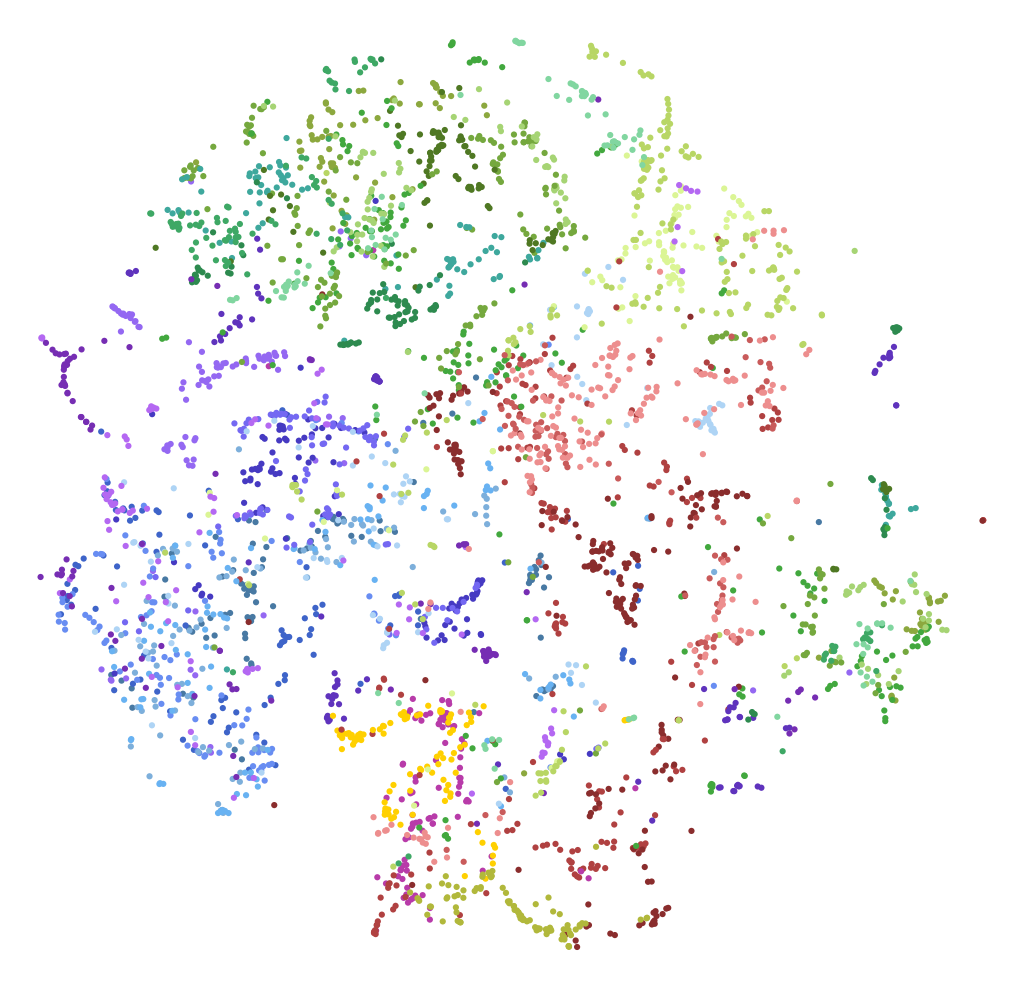
\includegraphics[width=\textwidth]{instruments-tsne.png}
%	\caption{A 2-D t-SNE embedding of sounds from Vienna Symphonic Library shows that a convolutional neural network can learn a manifold that separates the sounds of woodwinds (blue colors), strings (red colors), and brass (green colors) instruments.}\label{fig:tsne}
%\end{figure}




